\setcounter{definition}{0} \setcounter{property}{0} \setcounter{claim}{0} \setcounter{fact}{0} \setcounter{corollary}{0} \setcounter{figure}{0}
\section{Hierarchy of Complexity Classes and co-NP}

Recall that P stands for the set of decision problems that are polynomial-time solvable,
and NP stands for the set of decision problems that are polynomial-time verifiable.
Clearly, P is a subset of NP, i.e., P{}~$\subset${}~NP.
But is the case that P{}~$\neq${}~NP~(i.e., P is a strict subset of NP),
or P{}~$=${}~NP?  This question remains open,
and is perhap \emph{the} most important open question in computer science.
%(It is also one of the seven Millennium Prize Problems selected by the Clay Mathematics Institute.)

The existence of NP-complete problems gives a way to prove that P{}~$=${}~NP, by just showing
one NP-complete problem is polynomial-time solvable. This is intuitive: NP-complete
problems are the hardest problems in NP; if one of them is polynomial-time solvable,
then every problem must be polynomial-time solvable. We formally state it and prove it below.

\begin{fact}
Let $X$ be a NP-complete problem. If $X$ is in P, then P{}~$=${}~NP.
\end{fact}
\emph{Proof.} 	
In order to show P{}~$=${}~NP, we only need to prove NP{}~$\subset${}~P, as we already have P{}~$\subset${}~NP. 
Let $X'$ be an arbitrary problem in NP.  
Since $X$ is NP-complete, by definition, we know that $X'\le_p X$. Because
$X$ is in P, then we have that $X'$ is in P as well.
This proves that NP{}~$\subset${}~P, as $X'$ is arbitrary.  \qed

We define \emph{complementary} problem. Let $X$ be a decision problem.
Recall that $X$ is equivalently defined by all its instances, each of which
has a truth~(i.e., true of false). The \emph{complementary problem} of $X$,
denoted as $\overline{X}$, has the same set of instances with $X$ but each instance has an opposite truth.
See Figure~\ref{fig:co-np}.

\begin{figure}[!h]
\centering{

\tikzset{every picture/.style={line width=0.75pt}} %set default line width to 0.75pt        

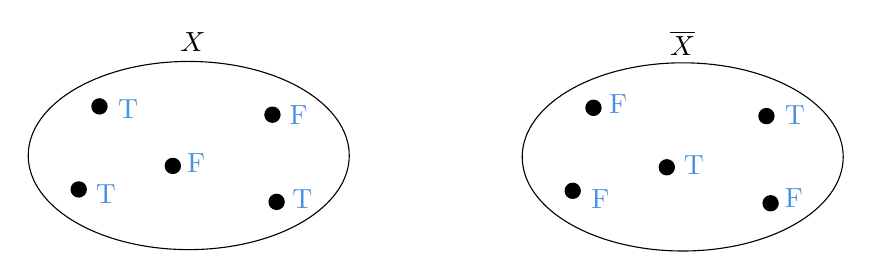
\begin{tikzpicture}[x=0.5pt,y=0.5pt,yscale=-1,xscale=1]
%uncomment if require: \path (0,300); %set diagram left start at 0, and has height of 300

%Shape: Ellipse [id:dp83662970590991] 
\draw   (8,96) .. controls (8,58.44) and (59.93,28) .. (124,28) .. controls (188.07,28) and (240,58.44) .. (240,96) .. controls (240,133.56) and (188.07,164) .. (124,164) .. controls (59.93,164) and (8,133.56) .. (8,96) -- cycle ;
%Shape: Circle [id:dp21341271480775648] 
\draw  [fill={rgb, 255:red, 0; green, 0; blue, 0 }  ,fill opacity=1 ] (54,60.5) .. controls (54,57.46) and (56.46,55) .. (59.5,55) .. controls (62.54,55) and (65,57.46) .. (65,60.5) .. controls (65,63.54) and (62.54,66) .. (59.5,66) .. controls (56.46,66) and (54,63.54) .. (54,60.5) -- cycle ;
%Shape: Circle [id:dp9929729618619046] 
\draw  [fill={rgb, 255:red, 0; green, 0; blue, 0 }  ,fill opacity=1 ] (39,120.5) .. controls (39,117.46) and (41.46,115) .. (44.5,115) .. controls (47.54,115) and (50,117.46) .. (50,120.5) .. controls (50,123.54) and (47.54,126) .. (44.5,126) .. controls (41.46,126) and (39,123.54) .. (39,120.5) -- cycle ;
%Shape: Circle [id:dp9620303268103491] 
\draw  [fill={rgb, 255:red, 0; green, 0; blue, 0 }  ,fill opacity=1 ] (107,103.5) .. controls (107,100.46) and (109.46,98) .. (112.5,98) .. controls (115.54,98) and (118,100.46) .. (118,103.5) .. controls (118,106.54) and (115.54,109) .. (112.5,109) .. controls (109.46,109) and (107,106.54) .. (107,103.5) -- cycle ;
%Shape: Circle [id:dp41706992941659915] 
\draw  [fill={rgb, 255:red, 0; green, 0; blue, 0 }  ,fill opacity=1 ] (179,66.5) .. controls (179,63.46) and (181.46,61) .. (184.5,61) .. controls (187.54,61) and (190,63.46) .. (190,66.5) .. controls (190,69.54) and (187.54,72) .. (184.5,72) .. controls (181.46,72) and (179,69.54) .. (179,66.5) -- cycle ;
%Shape: Circle [id:dp3550007068634743] 
\draw  [fill={rgb, 255:red, 0; green, 0; blue, 0 }  ,fill opacity=1 ] (182,129.5) .. controls (182,126.46) and (184.46,124) .. (187.5,124) .. controls (190.54,124) and (193,126.46) .. (193,129.5) .. controls (193,132.54) and (190.54,135) .. (187.5,135) .. controls (184.46,135) and (182,132.54) .. (182,129.5) -- cycle ;
%Shape: Ellipse [id:dp7490220245457752] 
\draw   (365,97) .. controls (365,59.44) and (416.93,29) .. (481,29) .. controls (545.07,29) and (597,59.44) .. (597,97) .. controls (597,134.56) and (545.07,165) .. (481,165) .. controls (416.93,165) and (365,134.56) .. (365,97) -- cycle ;
%Shape: Circle [id:dp3244374133914285] 
\draw  [fill={rgb, 255:red, 0; green, 0; blue, 0 }  ,fill opacity=1 ] (411,61.5) .. controls (411,58.46) and (413.46,56) .. (416.5,56) .. controls (419.54,56) and (422,58.46) .. (422,61.5) .. controls (422,64.54) and (419.54,67) .. (416.5,67) .. controls (413.46,67) and (411,64.54) .. (411,61.5) -- cycle ;
%Shape: Circle [id:dp41954634695015547] 
\draw  [fill={rgb, 255:red, 0; green, 0; blue, 0 }  ,fill opacity=1 ] (396,121.5) .. controls (396,118.46) and (398.46,116) .. (401.5,116) .. controls (404.54,116) and (407,118.46) .. (407,121.5) .. controls (407,124.54) and (404.54,127) .. (401.5,127) .. controls (398.46,127) and (396,124.54) .. (396,121.5) -- cycle ;
%Shape: Circle [id:dp7290812606891363] 
\draw  [fill={rgb, 255:red, 0; green, 0; blue, 0 }  ,fill opacity=1 ] (464,104.5) .. controls (464,101.46) and (466.46,99) .. (469.5,99) .. controls (472.54,99) and (475,101.46) .. (475,104.5) .. controls (475,107.54) and (472.54,110) .. (469.5,110) .. controls (466.46,110) and (464,107.54) .. (464,104.5) -- cycle ;
%Shape: Circle [id:dp4565505523195048] 
\draw  [fill={rgb, 255:red, 0; green, 0; blue, 0 }  ,fill opacity=1 ] (536,67.5) .. controls (536,64.46) and (538.46,62) .. (541.5,62) .. controls (544.54,62) and (547,64.46) .. (547,67.5) .. controls (547,70.54) and (544.54,73) .. (541.5,73) .. controls (538.46,73) and (536,70.54) .. (536,67.5) -- cycle ;
%Shape: Circle [id:dp8662075700047863] 
\draw  [fill={rgb, 255:red, 0; green, 0; blue, 0 }  ,fill opacity=1 ] (539,130.5) .. controls (539,127.46) and (541.46,125) .. (544.5,125) .. controls (547.54,125) and (550,127.46) .. (550,130.5) .. controls (550,133.54) and (547.54,136) .. (544.5,136) .. controls (541.46,136) and (539,133.54) .. (539,130.5) -- cycle ;

% Text Node
\draw (116,5) node [anchor=north west][inner sep=0.75pt]   [align=left] {$\displaystyle X$};
% Text Node
\draw (470,4) node [anchor=north west][inner sep=0.75pt]   [align=left] {$\displaystyle \overline{X}$};
% Text Node
\draw (71,54) node [anchor=north west][inner sep=0.75pt]  [color={rgb, 255:red, 74; green, 144; blue, 226 }  ,opacity=1 ] [align=left] {T};
% Text Node
\draw (121,93) node [anchor=north west][inner sep=0.75pt]  [color={rgb, 255:red, 74; green, 144; blue, 226 }  ,opacity=1 ] [align=left] {F};
% Text Node
\draw (426,50) node [anchor=north west][inner sep=0.75pt]  [color={rgb, 255:red, 74; green, 144; blue, 226 }  ,opacity=1 ] [align=left] {F};
% Text Node
\draw (553,118) node [anchor=north west][inner sep=0.75pt]  [color={rgb, 255:red, 74; green, 144; blue, 226 }  ,opacity=1 ] [align=left] {F};
% Text Node
\draw (195,58) node [anchor=north west][inner sep=0.75pt]  [color={rgb, 255:red, 74; green, 144; blue, 226 }  ,opacity=1 ] [align=left] {F};
% Text Node
\draw (413,119) node [anchor=north west][inner sep=0.75pt]  [color={rgb, 255:red, 74; green, 144; blue, 226 }  ,opacity=1 ] [align=left] {F};
% Text Node
\draw (55,115) node [anchor=north west][inner sep=0.75pt]  [color={rgb, 255:red, 74; green, 144; blue, 226 }  ,opacity=1 ] [align=left] {T};
% Text Node
\draw (197,119) node [anchor=north west][inner sep=0.75pt]  [color={rgb, 255:red, 74; green, 144; blue, 226 }  ,opacity=1 ] [align=left] {T};
% Text Node
\draw (480,94) node [anchor=north west][inner sep=0.75pt]  [color={rgb, 255:red, 74; green, 144; blue, 226 }  ,opacity=1 ] [align=left] {T};
% Text Node
\draw (553,58) node [anchor=north west][inner sep=0.75pt]  [color={rgb, 255:red, 74; green, 144; blue, 226 }  ,opacity=1 ] [align=left] {T};


\end{tikzpicture}

}
\caption{Illustration of problem $X$ and its complementary $\overline{X}$.}
\label{fig:co-np}
\end{figure}

For example, for 3SAT problem, an instance of 3SAT is a true instance if and only 
if there exists a truth assignment for variables such as all clauses can be satisfied.
Its complementary, $\overline{\textrm{3SAT}}$, still takes a set of variables and a set of clauses
as input. An instance of $\overline{\textrm{3SAT}}$ is a false instance if and only if
there exists a truth assignment for variables such as all clauses can be satisfied.

It is clear that, $\overline{\overline{X}} = X$. Another fact is: 
\begin{fact}
If $X$ is in P, then $\overline{X}$ is also in P. 
\label{fac:np1}
\end{fact}
This is because the polynomial-time algorithm
for $X$ essentially solves $\overline{X}$, by returning the opposite answer.

%Does $X \in \textrm{NP}$ imply that $\overline{X} \in \textrm{NP}$?
%This is complicated. In fact, this question remains open.
%Recall that, 
NP can also be described as the set of decision problems
with polynomial-size certificate for true instances.
We now introduce \emph{co-NP}, which is the set of decision problems
with polynomial-size certificate for false instances.
We formally define it below. It should be compared with the definition of NP.


\begin{definition}[co-NP]
Let $X$ be a decision problem. We say $X\in \textrm{co-NP}$ if there exists a polynomial-time algorithm $A$~(we call $A$ as a \emph{verifier}), such that,\\
        (1), verifier $A$ takes an instance $x$ of $X$ \emph{and} a polynomial-length certificate $c$ as input, and \\
        (2), for every instance $x$ of problem $X$: \\
        \hspace*{0.2cm} if $x$ is a ``false''-instance, then there must exist a certificate $c$ such that $A(x,c)$ returns ``no'';\\
        \hspace*{0.2cm} if $x$ is a ``true''-instance, then for any polynomial-length certificate $c$, $A(x,c)$ always returns ``yes''.
\end{definition}

By defintions of complementary problem and co-NP, we immediately have:
\begin{fact}
A decision problem $X$ is in NP if and only if $\overline{X}$ is in co-NP.
\label{fac:np2}
\end{fact}

%(The definition of co-NP can be regarded as another definition of complementary problems.)
We have shown that, if $X$ is in P then $\overline{X}$ is also in P. 
This implies that P is also a subset of co-NP. (Proof: let $X$ be an arbitrary problem in P.
So $\overline{X}$ is in P, which gives $\overline{X}$ is in NP; hence $X$ is in co-NP.)
Combining the fact that P is a subset of NP. We have

\begin{fact}
$\textrm{P} \subset \textrm{NP} \cap \textrm{co-NP}$.
\end{fact}

A natural question: is P equal to $\textrm{NP} \cap \textrm{co-NP}$, or P is a strict subset of 
$\textrm{NP} \cap \textrm{co-NP}$? This question remains open.
Another question: is NP equal to co-NP? This one remains open too. But we can prove the following.

\begin{fact}
If $\textrm{P} = \textrm{NP}$, then $\textrm{NP} = \textrm{co-NP}$.
\end{fact}

\emph{Proof.} Let $X$ be an arbitrary problem in NP. Since 
$\textrm{P} = \textrm{NP}$, we have $X$ is also in P.
According to Fact~\ref{fac:np1}, we know $\overline{X}$ is in P and hence also in NP.
Based on Fact~\ref{fac:np2}, we have $X\in \textrm{co-NP}$. This proves that $\textrm{NP}\subset \textrm{co-NP}$.
To prove the other side, let $X$ be an arbitrary problem in co-NP.
Hence, $\overline{X} \in \textrm{NP}$ and also $\overline{X} \in \textrm{P}$ because of the condition.
Again based on Fact~\ref{fac:np1}, we have $X$ is in P and therefore also in NP. 
This proves that $\textrm{co-NP}\subset \textrm{NP}$. \qed


See Figure~\ref{fig:hierarchy} for a hierarchy for the classes we have introduced,
depending on the possible results of 3 critical open questions in computer science.

\begin{figure}[!h]
\centering{

\tikzset{every picture/.style={line width=0.75pt}} %set default line width to 0.75pt        

\begin{tikzpicture}[x=0.58pt,y=0.58pt,yscale=-1,xscale=1]
%uncomment if require: \path (0,489); %set diagram left start at 0, and has height of 489

%Shape: Ellipse [id:dp9714732770479797] 
\draw   (22,140.42) .. controls (22,121.87) and (66.77,106.83) .. (122,106.83) .. controls (177.23,106.83) and (222,121.87) .. (222,140.42) .. controls (222,158.97) and (177.23,174.01) .. (122,174.01) .. controls (66.77,174.01) and (22,158.97) .. (22,140.42) -- cycle ;
%Straight Lines [id:da9470856219208896] 
\draw    (284,60) -- (176.77,104.84) ;
\draw [shift={(174,106)}, rotate = 337.31] [fill={rgb, 255:red, 0; green, 0; blue, 0 }  ][line width=0.08]  [draw opacity=0] (10.72,-5.15) -- (0,0) -- (10.72,5.15) -- (7.12,0) -- cycle    ;
%Shape: Ellipse [id:dp39391125687327155] 
\draw   (163,214.91) .. controls (163,194.43) and (207.77,177.83) .. (263,177.83) .. controls (318.23,177.83) and (363,194.43) .. (363,214.91) .. controls (363,235.4) and (318.23,252) .. (263,252) .. controls (207.77,252) and (163,235.4) .. (163,214.91) -- cycle ;
%Straight Lines [id:da6338019201234634] 
\draw    (401,141) -- (325.71,176.71) ;
\draw [shift={(323,178)}, rotate = 334.62] [fill={rgb, 255:red, 0; green, 0; blue, 0 }  ][line width=0.08]  [draw opacity=0] (10.72,-5.15) -- (0,0) -- (10.72,5.15) -- (7.12,0) -- cycle    ;
%Shape: Ellipse [id:dp13655633022849756] 
\draw   (262,215.54) .. controls (262,205.66) and (277.78,197.66) .. (297.25,197.66) .. controls (316.72,197.66) and (332.5,205.66) .. (332.5,215.54) .. controls (332.5,225.42) and (316.72,233.42) .. (297.25,233.42) .. controls (277.78,233.42) and (262,225.42) .. (262,215.54) -- cycle ;
%Shape: Ellipse [id:dp5449944288813106] 
\draw   (183,215.54) .. controls (183,205.66) and (198.78,197.66) .. (218.25,197.66) .. controls (237.72,197.66) and (253.5,205.66) .. (253.5,215.54) .. controls (253.5,225.42) and (237.72,233.42) .. (218.25,233.42) .. controls (198.78,233.42) and (183,225.42) .. (183,215.54) -- cycle ;
%Straight Lines [id:da030702262544070935] 
\draw    (317,61) -- (408.27,102.75) ;
\draw [shift={(411,104)}, rotate = 204.58] [fill={rgb, 255:red, 0; green, 0; blue, 0 }  ][line width=0.08]  [draw opacity=0] (10.72,-5.15) -- (0,0) -- (10.72,5.15) -- (7.12,0) -- cycle    ;
%Straight Lines [id:da1564630306712015] 
\draw    (434,142) -- (518.27,180.75) ;
\draw [shift={(521,182)}, rotate = 204.69] [fill={rgb, 255:red, 0; green, 0; blue, 0 }  ][line width=0.08]  [draw opacity=0] (10.72,-5.15) -- (0,0) -- (10.72,5.15) -- (7.12,0) -- cycle    ;
%Shape: Ellipse [id:dp6368613727912615] 
\draw   (289,308.91) .. controls (289,290.09) and (327.28,274.83) .. (374.5,274.83) .. controls (421.72,274.83) and (460,290.09) .. (460,308.91) .. controls (460,327.74) and (421.72,343) .. (374.5,343) .. controls (327.28,343) and (289,327.74) .. (289,308.91) -- cycle ;
%Shape: Ellipse [id:dp08483334028737277] 
\draw   (305,312.54) .. controls (305,302.66) and (320.78,294.66) .. (340.25,294.66) .. controls (359.72,294.66) and (375.5,302.66) .. (375.5,312.54) .. controls (375.5,322.42) and (359.72,330.42) .. (340.25,330.42) .. controls (320.78,330.42) and (305,322.42) .. (305,312.54) -- cycle ;
%Shape: Ellipse [id:dp4660930800548526] 
\draw   (389,309) .. controls (389,290.22) and (420.79,275) .. (460,275) .. controls (499.21,275) and (531,290.22) .. (531,309) .. controls (531,327.78) and (499.21,343) .. (460,343) .. controls (420.79,343) and (389,327.78) .. (389,309) -- cycle ;
%Straight Lines [id:da5096569303441225] 
\draw    (515,220) -- (423.68,265.66) ;
\draw [shift={(421,267)}, rotate = 333.43] [fill={rgb, 255:red, 0; green, 0; blue, 0 }  ][line width=0.08]  [draw opacity=0] (10.72,-5.15) -- (0,0) -- (10.72,5.15) -- (7.12,0) -- cycle    ;
%Shape: Ellipse [id:dp5549354135393528] 
\draw   (594,307.91) .. controls (594,289.09) and (630.71,273.83) .. (676,273.83) .. controls (721.29,273.83) and (758,289.09) .. (758,307.91) .. controls (758,326.74) and (721.29,342) .. (676,342) .. controls (630.71,342) and (594,326.74) .. (594,307.91) -- cycle ;
%Shape: Ellipse [id:dp22039734942458056] 
\draw   (608,311.54) .. controls (608,301.66) and (623.78,293.66) .. (643.25,293.66) .. controls (662.72,293.66) and (678.5,301.66) .. (678.5,311.54) .. controls (678.5,321.42) and (662.72,329.42) .. (643.25,329.42) .. controls (623.78,329.42) and (608,321.42) .. (608,311.54) -- cycle ;
%Shape: Ellipse [id:dp5560061601595019] 
\draw   (687,308) .. controls (687,289.22) and (714.31,274) .. (748,274) .. controls (781.69,274) and (809,289.22) .. (809,308) .. controls (809,326.78) and (781.69,342) .. (748,342) .. controls (714.31,342) and (687,326.78) .. (687,308) -- cycle ;
%Straight Lines [id:da6023491908932058] 
\draw    (572,219) -- (674.24,262.82) ;
\draw [shift={(677,264)}, rotate = 203.2] [fill={rgb, 255:red, 0; green, 0; blue, 0 }  ][line width=0.08]  [draw opacity=0] (10.72,-5.15) -- (0,0) -- (10.72,5.15) -- (7.12,0) -- cycle    ;
%Shape: Ellipse [id:dp055919448535677874] 
\draw   (701,309.33) .. controls (701,297.91) and (710.63,288.66) .. (722.5,288.66) .. controls (734.37,288.66) and (744,297.91) .. (744,309.33) .. controls (744,320.74) and (734.37,330) .. (722.5,330) .. controls (710.63,330) and (701,320.74) .. (701,309.33) -- cycle ;

% Text Node
\draw    (265,22.5) -- (329,22.5) -- (329,60.5) -- (265,60.5) -- cycle  ;
\draw (268,26.5) node [anchor=north west][inner sep=0.75pt]   [align=left] {P $\displaystyle \overset{?}{=}$NP};
% Text Node
\draw (36,133.5) node [anchor=north west][inner sep=0.75pt]   [align=left] {P $\displaystyle =$NP$\displaystyle =$co-NP$\displaystyle =$NPC};
% Text Node
\draw    (368,103.5) -- (464,103.5) -- (464,141.5) -- (368,141.5) -- cycle  ;
\draw (371,107.5) node [anchor=north west][inner sep=0.75pt]   [align=left] {NP $\displaystyle \overset{?}{=}$co-NP};
% Text Node
\draw (218,250.5) node [anchor=north west][inner sep=0.75pt]   [align=left] {NP$\displaystyle =$co-NP};
% Text Node
\draw (292.12,208.56) node [anchor=north west][inner sep=0.75pt]   [align=left] {P};
% Text Node
\draw (202.12,207.56) node [anchor=north west][inner sep=0.75pt]   [align=left] {NPC};
% Text Node
\draw    (478,181.5) -- (602,181.5) -- (602,219.5) -- (478,219.5) -- cycle  ;
\draw (481,185.5) node [anchor=north west][inner sep=0.75pt]   [align=left] {P $\displaystyle \overset{?}{=}$NP$\displaystyle \cap $co-NP};
% Text Node
\draw (363,344.5) node [anchor=north west][inner sep=0.75pt]   [align=left] {NP};
% Text Node
\draw (420.12,303.56) node [anchor=north west][inner sep=0.75pt]   [align=left] {P};
% Text Node
\draw (324.12,304.56) node [anchor=north west][inner sep=0.75pt]   [align=left] {NPC};
% Text Node
\draw (444,345.5) node [anchor=north west][inner sep=0.75pt]   [align=left] {co-NP};
% Text Node
\draw (665,343.5) node [anchor=north west][inner sep=0.75pt]   [align=left] {NP};
% Text Node
\draw (718.12,302.56) node [anchor=north west][inner sep=0.75pt]   [align=left] {P};
% Text Node
\draw (627.12,303.56) node [anchor=north west][inner sep=0.75pt]   [align=left] {NPC};
% Text Node
\draw (730,343.5) node [anchor=north west][inner sep=0.75pt]   [align=left] {co-NP};
% Text Node
\draw (211,65) node [anchor=north west][inner sep=0.75pt]   [align=left] {Y};
% Text Node
\draw (363,64) node [anchor=north west][inner sep=0.75pt]   [align=left] {N};
% Text Node
\draw (346,146) node [anchor=north west][inner sep=0.75pt]   [align=left] {Y};
% Text Node
\draw (446,231) node [anchor=north west][inner sep=0.75pt]   [align=left] {Y};
% Text Node
\draw (482,145) node [anchor=north west][inner sep=0.75pt]   [align=left] {N};
% Text Node
\draw (629,225) node [anchor=north west][inner sep=0.75pt]   [align=left] {N};


\end{tikzpicture}

}
\caption{Hierarchy of the complexity classes. All 3 questions in the boxes are open.}
\label{fig:hierarchy}
\end{figure}

You might wonder, in the fourth situation shown in Figure~\ref{fig:hierarchy},
whether it is possible for NPC and co-NP to overlap. The answer is no; the reason is stated below.
Its proof uses this conclusion~(that we do not prove): if $A \le_p B$ and $B\in\textrm{NP}$ then $A\in\textrm{NP}$. 

\begin{fact}
Let $X$ be NP-complete. If $X$ is in co-NP, then $\textrm{NP} = \textrm{co-NP}$.
\label{fac:np3}
\end{fact}
\emph{Proof.} Let $X'$ be an arbitrary problem in NP.
Since $X$ is NP-complete, we have $X' \le_p X$, i.e., we can design an
algorithm for $X'$ using polynomial number of calls of a solver for $X$.
This algorithm for $X'$, when modified to return the opporsite answer, exactly solves $\overline{X'}$.
This implies that $\overline{X'} \le_p X$. 
Since $X\in\textrm{NP}$, according to the said conclusion,
we have $\overline{X'}\in\textrm{NP}$ which gives $X'\in\textrm{co-NP}$.
This proves that $\textrm{NP}\subset \textrm{co-NP}$.
To prove the other side, let $X'$ be an arbitrary problem in co-NP, which gives $\overline{X'} \in \textrm{NP}$.
Hence, $\overline{X'} \le_p X$. Using the same argument, we have $X'\le_p X$.
Using above conclusion and that $X\in \textrm{NP}$, we have $X'\in\textrm{NP}$.
This proves that $\textrm{co-NP}\subset\textrm{NP}$. \qed

\subsection*{Interger Factorization}

For all NP-complete problems we have seen, %so far, such as 3SAT, $IS(G, k)$, and perfect 3D matching,
their true instances are in the form of ``there exists an object''.
For examples, a 3SAT instance is true if there exists an truth assignment that satisfies all clauses;
an $IS(G, k)$ instance is true if there exists an independent set of size at least $k$;
a perfect 3D matching instance is true if there exists a perfect matching.
It is therefore straightforward to show that these problems are in NP,
as NP requires a (polynomial-size) certificate for true instances, and
the ``object'' naturally serves as such a certificate.
In contrast, their false instances are in the form of 
``there does not exist an object''. As a result, it is much more difficult, or even impossible,
to prove that these problems are in co-NP, as it requires a polynomial-size certificate for false instances. 
In fact, none of these NP-complete is known to be in co-NP~(as otherwise NP will be equal to co-NP, according
to Fact~\ref{fac:np3}).

Any problem in P is known to be both in NP and co-NP.
Is there a problem that is not known to be in P, but in both NP and co-NP?
We introduce such a problem now, the \emph{interger factorization problem}. 
This problem takes two positive integers $X$ and $t$ as input,
and seeks if there exists a factor $a$ of $X$ such that $a\le t$.
(Recall that $a$ is a factor of $X$ means $X$ is divisible $a$, or equivalently, $X \textrm{ mod } a = 0$.)

You might think this problem can be solved in polynomial-time. Consider the following:

\begin{algorithmblock}[0.8\textwidth]
        \aaA {4}{algorithm-for-integer-factorization~($X,t$)}\xxx
        \aaB {2}{for $a = 2 \to t$}\xxx
        \aac {if $X \textrm{ mod } a = 0$: return ``yes''}\xxx
        \aab {return ``no'';}\xxx
\end{algorithmblock}

This algorithm is certainly correct, but it runs in exponential time.
Recall that runtime is a function of input size.
For this problem, the input is $X$ and $t$ and the input size
is the number of bits storing them, which are $\log X$ and $\log t$ respectively.
Let $m = \log X$ and $n = \log t$.
Computing $X \textrm{ mod } a$ takes $O(\log X \cdot \log a) = O(mn)$ time.
The entire algorithm takes $O(tmn) = O(mn2^n)$ time, which is exponential.

We first show that this problem in NP. It is again easy.
%It is again easy to show that the interger factorization problem is in NP.
The certificate is simply a factor of $X$ that is less than or equal to $t$.
Specifically, the verifier takes $X$, $t$, and certificate $c$ as input,
and verifies whether $X \textrm{ mod } c = 0$ and whether $c \le t$.

Proving that this problem is in co-NP is more complicated and more interesting.
An instance is false if all factors of $X$ are greater than $t$.
Using all factors as certificate does not work, as its size is exponential: 
there are $O(X) = O(2^m)$ number of factors.
The key idea is, we only need to check \emph{prime} factors: all factors of $X$ are greater than $t$
if and only if all prime factors of $X$ are greater than $t$.

The number of prime factors of integer $X$ is $O(m)$. To see this, consider the factorization of $X$:
$$X = \Pi_{i=1}^k p_i^{n_i},$$
where $p_i$ is a prime and $n_i \ge 1$. The distinct number of prime factors of $X$ is $k$.
To show that $k = O(m)$, take logarithm on both sides:
%\begin{eqnarray*}
$$\log X = \sum_{i=1}^k n_i \log p_i \ge \sum_{i=1}^k \log p_i \ge \sum_{i=1}^k \log 2 = k\cdot \log 2,$$
which gives $k = O(\log X) = O(m)$.
%\end{eqnarray*}

We hence use a prime factorization, consisting of $k$ pairs $\{(p_i, n_i) \mid 1\le i \le k\}$, as a certificate for false instances.
The verifier takes $X$ and $t$ and certificate $c$ as input.
It verifies whether $c$ consists of pairs of numbers  $\{(p_i, n_i)\}$.
It then verifies whether $c$ gives a factorization of $X$, i.e., to verify $X = \Pi p_i^{n_i}$.
It also verifies whether $\{p_i\}$ are all primes and whether they are all greater than $t$.
The verifier returns ``no'' if all these pass, and otherwise return ``yes''.

According to above analysis, an instance is false if all prime factors are greater than $t$. 
For a false instance, the certificate~(i.e., prime factors and their powers) is in polynomial size, which we have proved.
The verifier runs in polynomial-time. The only step that needs
attention is to verify $\{p_i\}$ are primes,
but thanks to the AKS algorithm~(2002), testing whether an integer is a prime can be done in polynomial-time.
This concludes the proof that the interger factorization problem is in co-NP.
